\section{Beispiele}
Diese Beispiele wurden in einer dafür konzipierten Erweiterung für das \name{mec-2} HTML Element gezeichnet.
Komplexere Modelle in einem Zug zu zeichnen ist mit den aktuellen Modellen noch mühselig, was zum einem daran liegt, dass die Trainingsdaten nicht mit dem selben Zeichenwerkzeug generiert wurden und zum anderen, dass die Modelle nicht robust genug trainiert sind, als das dies ein Problem darstellt.

\begin{figure}[H]
    \centering
    \begin{subfigure}[b]{0.3\textwidth}
        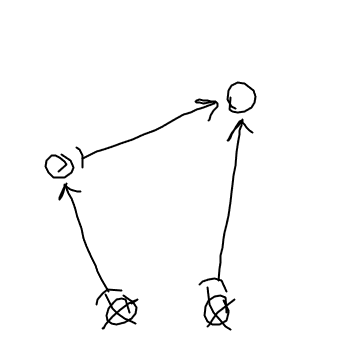
\includegraphics[width=\textwidth]{images/4bar_sketch.png}
        \caption{}
        \label{fig:4bar_sketch}
    \end{subfigure}
    \begin{subfigure}[b]{0.3\textwidth}
        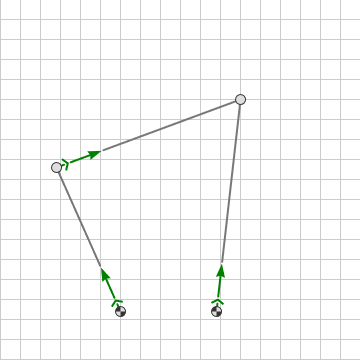
\includegraphics[width=\textwidth]{images/4bar_prediction.png}
        \caption{}
        \label{fig:4bar_prediction}
    \end{subfigure}
    \label{fig:4bar_example}
    \caption{Ein Viergelenk}
\end{figure}

\begin{figure}[H]
    \centering
    \begin{subfigure}[b]{0.3\textwidth}
        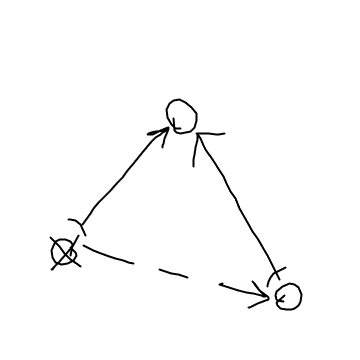
\includegraphics[width=\textwidth]{images/pump_sketch.png}
        \caption{}
        \label{fig:pump_sketch}
    \end{subfigure}
    \begin{subfigure}[b]{0.3\textwidth}
        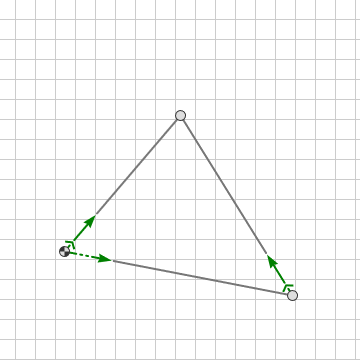
\includegraphics[width=\textwidth]{images/pump_prediction.png}
        \caption{}
        \label{fig:pump_prediction}
    \end{subfigure}
    \label{fig:pump_example}
    \caption{Mechanismus mit translatorischem Glied}
\end{figure}